% usage manual (6-10 pages)
\chapter{Ръководство на потребителя}
  \section{Сваляне на кода от интернет}
  Кодът на приложението и документацията е качен в GitHub и може да се свали локално чрез {\tt git} с командата показана във фигура \ref{fig:repo-download}.
  \begin{figure}[htpb]
    \centering
    \begin{minted}{bash}
      $ git clone --recurse-submodules https://github.com/umnikos/Bare-Metal-Encryption.git
    \end{minted}
    \caption{Сваляне на кода чрез {\tt git}}
    \label{fig:repo-download}
  \end{figure}

  \section{Компилиране на документацията}
  Документацията е написана на \LaTeX{}. Намира се в папка {\tt docs} и най-лесно се компилира с командите във фигура \ref{fig:latex-compiling}. Ако на машината липсват {\tt pdflatex} или {\tt bibtex} или се получават грешки при компилация то вероятно не са инсталирани всички нужни \LaTeX{} пакети. Инсталацията става по начинът, показан във фигура \ref{fig:latex-requirements}.
  % FIXME - minted changed the requirements!
  \begin{figure}[htpb]
    \centering
    \begin{minted}{bash}
      $ pdflatex -shell-escape docs.latex
      $ bibtex docs
      $ pdflatex -shell-escape docs.latex
      $ pdflatex -shell-escape docs.latex
    \end{minted}
    \caption{Компилиране на документацията (за Linux)}
    \label{fig:latex-compiling}
  \end{figure}
  \begin{figure}[htpb]
    \centering
    \begin{minted}{bash}
      $ sudo apt update
      $ sudo apt install texlive-latex-base texlive-lang-cyrillic texlive-latex-extra biber
    \end{minted}
    \caption{Инсталиране на нужните \LaTeX{} библиотеки (за Debian-базирани Linux дистрибуции)}
    \label{fig:latex-requirements}
  \end{figure}

  \section{Компилиране на приложението}
  Различни конфигурации на кода се намират в папка {\tt builds}. Пример за това как се компилира и изпълнява една от възможните конфигурации е даден във фигура \ref{fig:build-making}. Втората команда е за компилиране на кода, а третата команда е за изпълняване на кода чрез QEMU. QEMU се инсталира по начинът, показан във фигура \ref{fig:installing-qemu}.

  \begin{figure}[htpb]
    \centering
    \begin{minted}{bash}
      $ cd docs/bare-metal-encryption
      $ make main-serial
      $ make run-serial
    \end{minted}
    \caption{Компилиране и изпълняване на една от възможните конфигурации (за Linux)}
    \label{fig:build-making}
  \end{figure}

  \begin{figure}[htpb]
    \centering
    \begin{minted}{bash}
      $ sudo apt update
      $ sudo apt install qemu-system-x86
    \end{minted}
    \caption{Инсталиране на QEMU (за Debian-базирани Linux дистрибуции)}
    \label{fig:installing-qemu}
  \end{figure}

  За компилация е нужно да има инсталиран i686 C cross-compiler. Такъв компилатор не се предлага в {\tt apt} вече компилиран, а трябва да се компилира от сорс. За тази цел са нужни няколко програми, които се инсталират с командите, показани във фигура \ref{fig:gcc-requirements}.

  \begin{figure}[htpb]
    \centering
    \begin{minted}{bash}
      $ sudo apt update
      $ sudo apt install build-essential bison flex libgmp3-dev libmpc-dev libmpfr-dev texinfo
    \end{minted}
    \caption{Инсталиране на нужните програми за компилиране на GCC (за Debian-базирани Linux дистрибуции)}
    \label{fig:gcc-requirements}
  \end{figure}

  Сорс кодовете могат да бъдат изтеглени от {\tt https://ftp.gnu.org/gnu/gcc/} и {\tt https://ftp.gnu.org/gnu/binutils/} като {\tt .tar.gz} файлове. След свалянето на кода на {\tt gcc} и {\tt binutils} следва да бъдат компилирани с командите, показани във фигура \ref{fig:compiling-gcc}.
  {\tt TARGET} е мястото, където ще се инсталира компилатора и може да бъде променено. Тези команди трябва да се изпълнят в един и същи терминал в този ред.
  Трябва да се има предвид, че този процес може да отнеме време.

  \begin{figure}[htpb]
    \centering
    \begin{minted}{bash}
      $ export PREFIX="$HOME/opt/cross"
      $ export PATH="$PREFIX/bin:$PATH"
      $ export TARGET=i686-elf

      $ cd ~/Downloads
      $ tar zxf gcc-10.2.0.tar.gz
      $ tar zxf binutils-2.36.tar.gz

      $ mkdir build-binutils
      $ cd build-binutils
      $ ../binutils-2.36/configure --target=$TARGET --prefix="$PREFIX" --with-sysroot --disable-nls --disable-werror
      $ make
      $ make install

      $ cd ..
      $ mkdir build-gcc
      $ cd build-gcc
      $ ../gcc-10.2.0/configure --target=$TARGET --prefix="$PREFIX" --disable-nls --enable-languages=c,c++ --without-headers
      $ make all-gcc
      $ make all-target-libgcc
      $ make install-gcc
      $ make install-target-libgcc
    \end{minted}
    \caption{Компилиране на GCC като cross-compiler (за Linux)}
    \label{fig:compiling-gcc}
  \end{figure}

  Ако инсталацията е успешна трябва да бъде направена перманентна като се добави пътят към компилатора в {\tt \$PATH} променливата за постоянно. Това става като се редактира {\tt \~{}/.bashrc} файла. Фигура \ref{fig:adding-to-path} показва един от възможните начини това да се направи.

  \begin{figure}[htpb]
    \centering
    \begin{minted}{bash}
      $ echo 'export PATH="'$PREFIX'/bin:$PATH"' >> testfile.txt
    \end{minted}
    \caption{Добавяне на пътя до компилатора към {\tt \$PATH} променливата}
    \label{fig:adding-to-path}
  \end{figure}

  \section{Начин на ползване}
  След командата {\tt make run-serial} би трябвало да се появи нов прозорец който изглежда като този във фигура \ref{fig:qemu-window}. След натискането на {\tt Enter} клавиша от клавиатурата прозорецът ще стане чисто черен, но терминалът, от който е стартиран приложението, вече ще се е променил и ще изглежда като във фигура \ref{fig:interface-initial}.

  \begin{figure}[htpb]
    \centering
    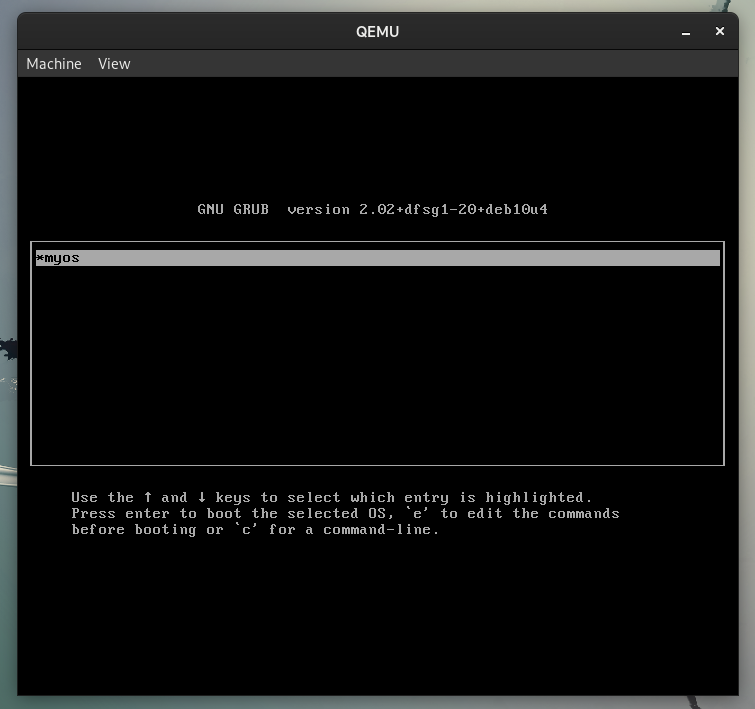
\includegraphics[width=\textwidth]{qemu-window}
    \caption{Прозорецът, създаден от QEMU}
    \label{fig:qemu-window}
  \end{figure}

  \begin{figure}[htpb]
    \centering
    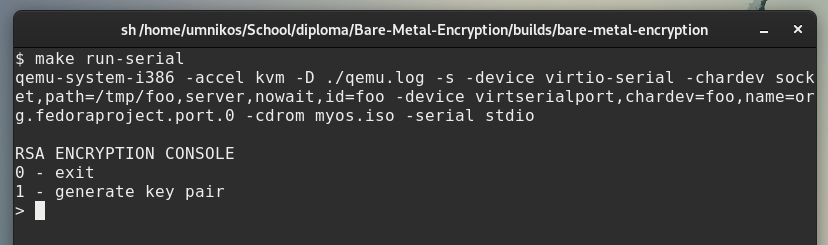
\includegraphics[width=\textwidth]{interface-initial}
    \caption{Първоначалното състояние на потребителския интерфейс}
    \label{fig:interface-initial}
  \end{figure}

